\subsection{Model Intuition} 
\label{sec:intuition}

Our model is inspired by the similar idea of collaborative filtering
that the preference of a user on an item is predicted based on the
preferences of other users with similar interests.  There are mainly
two categories of collaborative filtering, either in user-centric or
item-centric manner:
\begin{itemize}
\item item-based collaborative filtering: build an item-item matrix
  determining relationships between pairs of items, then infer the
  tastes of the current user by examining the matrix and matching that
  user's data, e.g. users who bought x also bought y
\item user-based collaborative filtering: look for users who share the
  same rating patterns with the active user (the user whom the
  prediction is for). Then use the ratings from those like-minded
  users found in step 1 to calculate a prediction for the active user,
  e.g. people also looks at the following items
\end{itemize}
Both item-based and user-based models are trying to emphasize only one
perspective of the problem, but did not consider the correlation cross
them.

\textit{ Is it possible to use the information from both dimensions to
  further improve the model's prediction performance? }

The answer is positive. We approach this problem by mining the
homogeneous similartiy across advertisement and keyword dimentions, in
another word, similarity ratio of different keywords between similar
advertisement should be close to each other.  Instead of using only
item-based or user-based method, it is a synthetic multi-dimension
model, which evaluates the similarity cross item and user
dimensions. Also, different from item-based or user-based method,
which uses a predefine static similarity function and calculate the
global optimal similarity, we are using a local optimal function,
which can dynamic involving similarity using learned parameters, hence
can support large scale data in an efficient computation cost.

The main idea of our model is illustrated by
Figure~\ref{fig:sppan-idea}, where $u,v,w$ are advertisements, and
$i,j,k$ are keywords, and the value in each cell is the average daily
clicks for the corresponding advertisement from the keyword query.
Let's say we want to predict the average daily click value if we want
to add keyword $k$ to advertisement $v$. For keyword pair $k$ and $j$,
we observed ratio $20/12$ in advertisement $u$ and $5/18$ in
advertisement $w$. If we can derive the performance ratio between $k$
and $j$ in advertisement $v$, then we can make use of $j$'s observed
daily average clicks in $v$ to give one estimate of $k$'s daily
average clicks in $v$. To do so, we introduce a set of parameters
called {\em similarity}, one for each pair of advertisements, to
capture how similar the performance ratios will be between
advertisements. Let $\similarity{u}{v},\similarity{v}{w}$ be the
similarity between $u,v$ and $v,w$ respectively. The estimate given by
keyword pair $k,j$ can be expressed as
\[ 6\times \left(\frac{20}{12}\times\similarity{u}{v} + \frac{5}{18}\times\similarity{v}{w} \right)\div \left(\similarity{u}{v} + \similarity{v}{w} \right) \]
Similarly, we can have another estimate by keyword pair $k,i$, which is
\[ 9\times \left(\frac{20}{5}\times\similarity{u}{v} + \frac{5}{22}\times\similarity{v}{w} \right)\div \left(\similarity{u}{v} + \similarity{v}{w} \right) \]

\begin{figure}[!ht]
  \centering
  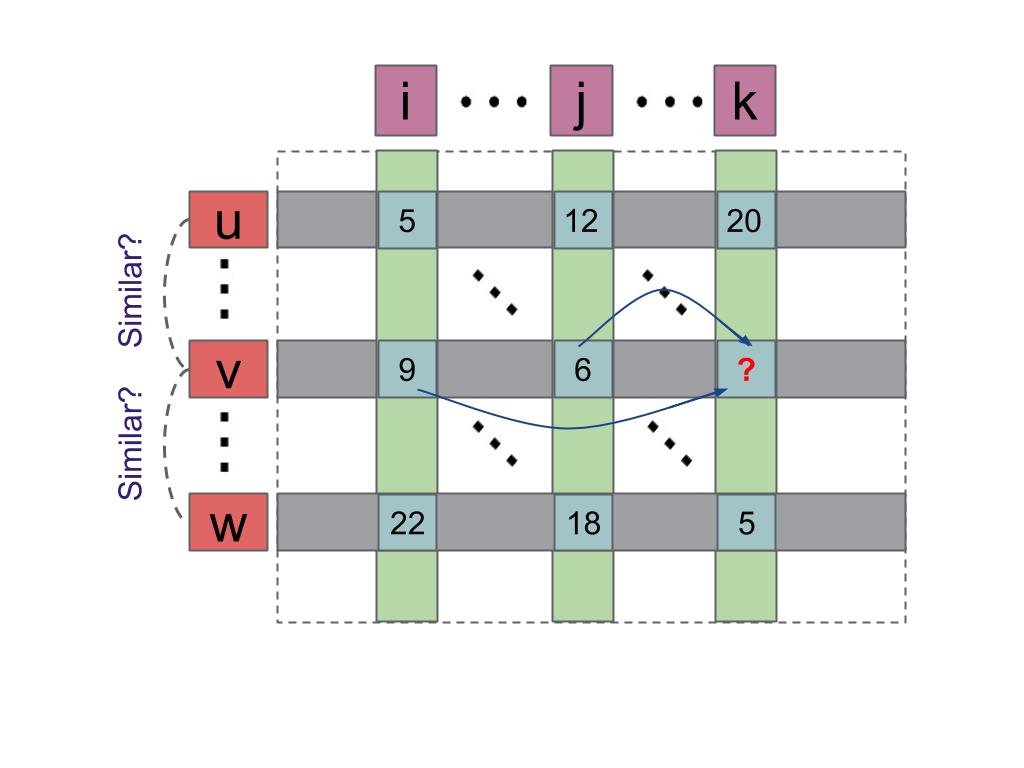
\includegraphics[width=0.5\textwidth]{figures/example.jpg}
  \caption{High level idea of {\sppan} model.}
  \label{fig:sppan-idea}
\end{figure}

Now how do we combine these estimates? We introduce another set of
parameters called {\em confidence}, one for each pair of
keywords. Therefore, the final estimate can be represented as the
linear combination of the above two estimates, weighted by the
confidences of keyword pairs $k,j$ and $k,i$. All the parameters are
learned from {\sppan} trainer defined in Section~\ref{sec:trainer}.
The details of parameters are covered in Section~\ref{sec:detail}.
